\paragraph{An Illustrative Example} 

The context of this work is in the oceanographic domain with an
autonomous underwater vehicle (AUV) with an illustrative issue arising
with dynamic goal emergence. The AUV can autonomously plan and execute
goals sent from shore. In this domain, an AUV can either transit from
one location to another within the water column, or survey a location
in order to collect data about a feature of interest; an example being
a hydrothermal vent depicted in Fig. \ref{fig:Example}.  Note that the
AUV must pass through {\em Vent1} to get to {\em Vent2}.  The vehicle
is deployed initially with the scientific objective of sampling {\em
  Vent 2} and the operational goal of being back at the {\em Surface} by
the end of the mission which lasts $12$ hours. The support ship can
send short commands to the AUV and receive limited data via acoustic
communications.  The traditional approach to such AUV surveys has been
to separate exploration and exploitation into two different surveys
\cite{Yoerger01012007}.  By improving how the vehicle handles the
inclusion of new goals, we can greatly improve the efficacy of such
surveys.

%%%%%%%%%%%%%%%%%%
% Use the following if really needed
% \subfloat[\small Bathymetry of vent sites off of NW United States]{\label{fig:ex:axial}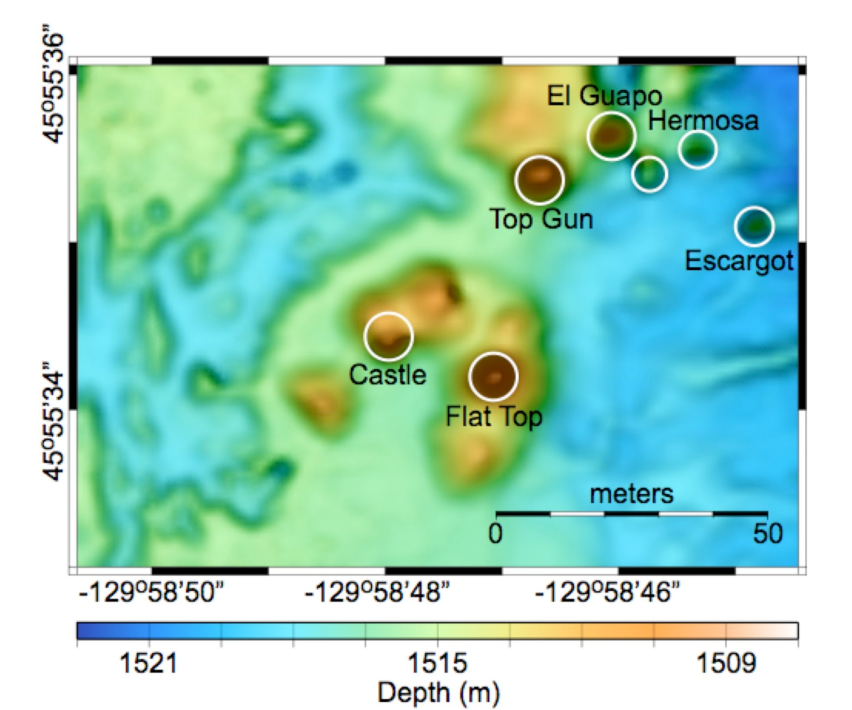
\includegraphics[scale=0.35]{figs/vents.pdf}}
%%%%%%%%%%%%%%%%%%
\begin{figure}[!t]
  \centering
  \vskip-3mm
  \subfloat[]{\label{fig:ex:graph}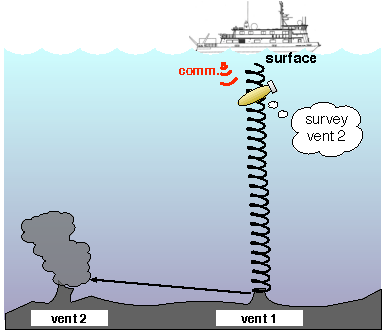
\includegraphics[width=0.45\columnwidth]{figs/auv_example}}
  \hfill \subfloat[] {\label{fig:ex:plan}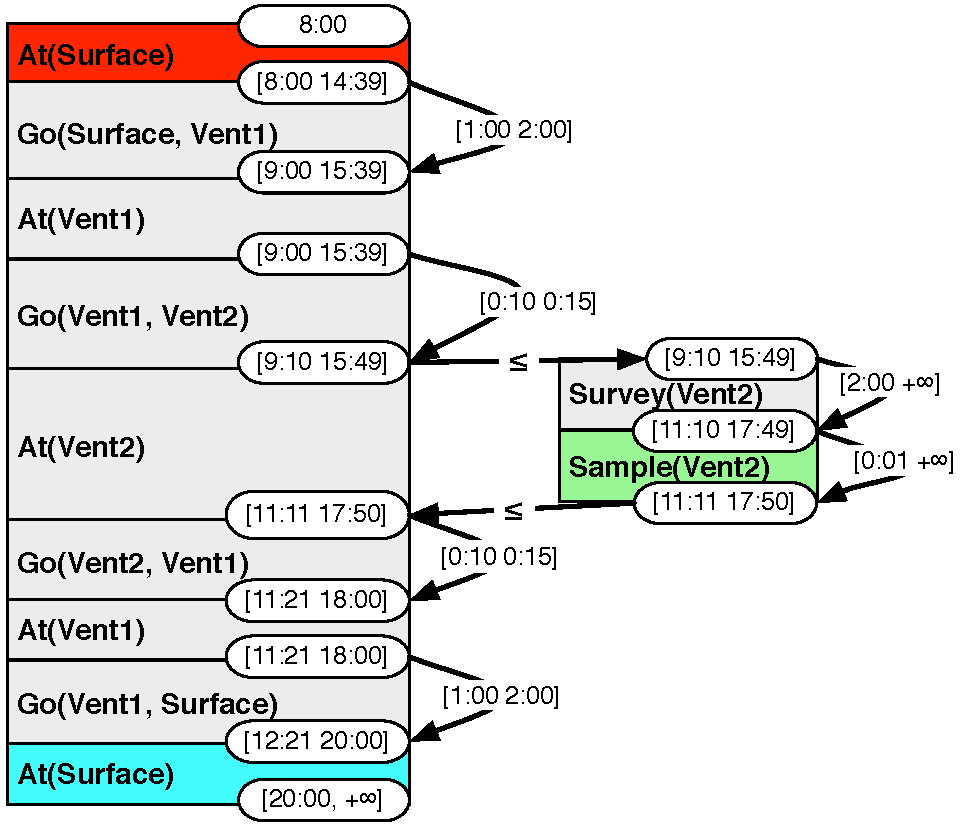
\includegraphics[width=0.55\columnwidth]{figs/example_plan}}
  %\hfill \subfloat[\small Initial planning problem.]{\label{fig:ex:init}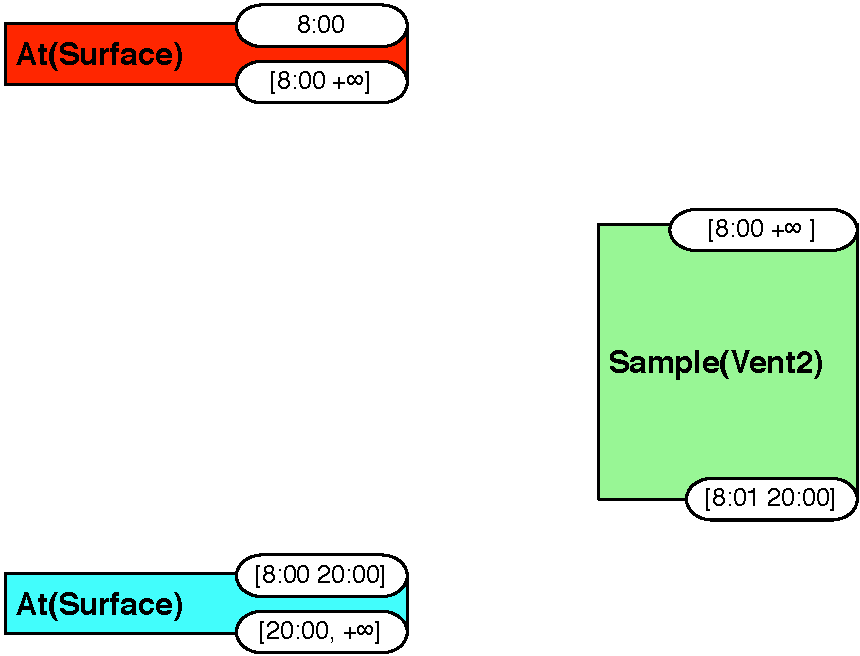
\includegraphics[width=0.49\columnwidth]{figs/example_initial}}
  \vskip-2mm
  \caption{\small{(\ref{fig:ex:graph}) illustrates the domain and
      (\ref{fig:ex:plan}) an initial plan for the problem. The AUV is
      initially at {\em Surface} at 8:00 and the mission is expected
      to complete by 20:00 with the goal --- marked with thick borders
      --- to sample {\em Vent 2} and the operational goal to be back
      at the surface for recovery by mission end.}}
  \label{fig:Example}
  \vskip-3mm
\end{figure}

Given the initial problem in Fig. \ref{fig:ex:graph}, the onboard
planner on the AUV produces the flexible temporal plan shown in
Fig. \ref{fig:ex:plan} for execution. However, at any time during the
mission scientists can decide, for example, that they also want to
{\em sample} {\em Vent 1} as a consequence of data processing during
the traverse from the surface to {\em Vent 2}.  Time on site for such
bathymetric exploration is limited and expensive, so dynamic goal
generation is a reality.  Finding a balance between executing a plan
action \emph{proactive}ly or waiting, is the dichotomy that the plan
executive needs to resolve. Not doing so impacts the mission
efficiency.

% . Otherwise, the plan will suffer along with
% the efficiency of the mission.

% This raises the issue of balancing the decisions during plan execution
% between staring one plan action as early as possible --- which we will
% call {\em proactive} -- or wait until the action should necessarily
% start -- called later. There is a clear difference between the two
% approaches but when should, for example, the AUV wait or start early
% and how either will impact the mission execution when the new
% objective will be integrated by the AUV ?

%\begin{figure}[!htb]
%  \centering
%  % \fcomment{In all the figures goals' color are the same "grey" as the
%  %   other actions .... need to correct this.}
%  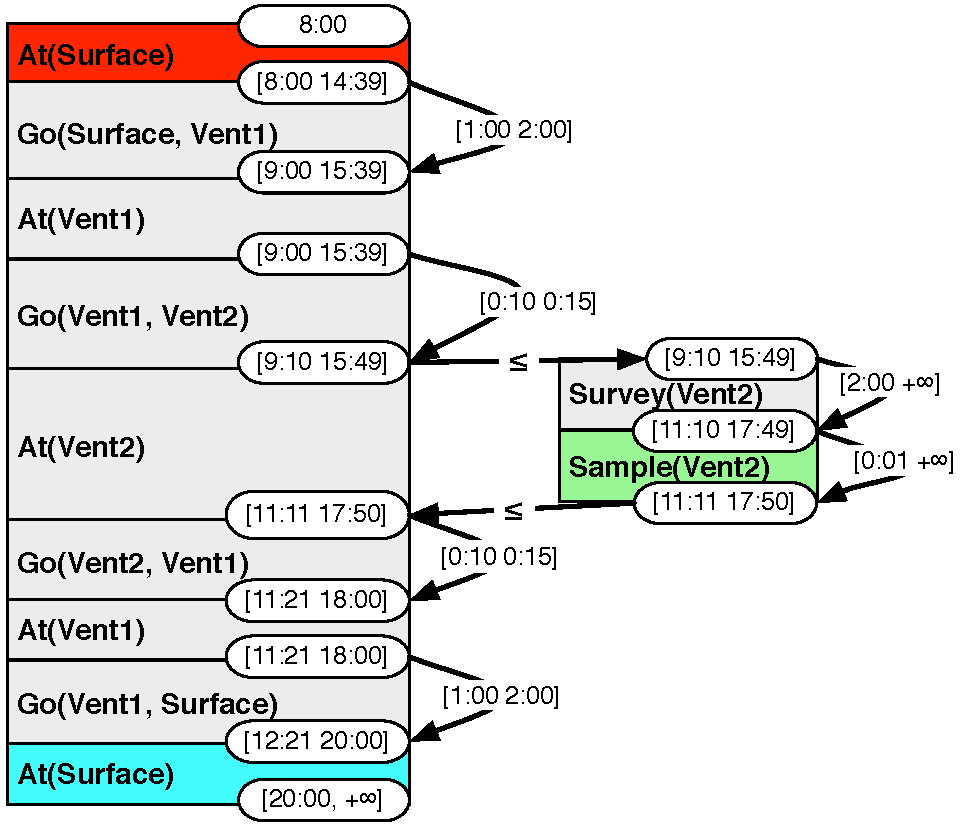
\includegraphics[width=0.8\columnwidth]{figs/example_plan}
%  \vskip-2mm
%  \caption{\small The flexible plan solution of the AUV domain in
%    Fig. \ref{fig:Example}}
%  \label{fig:ex:plan}
%\end{figure}

Exclusively {\em deferring} the actions is not acceptable since it
results in the vehicle sitting at the surface, diving only at the very
last minute. Subsequently, if a new goal arrives there is no time left
to execute outstanding objectives, leaving the robot to exclude one of
the goals or fail to be at the surface as planned by 20:00. Equally,
the {\em proactive} approach can be problematic, since the vehicle
will go through the actions of the plan and be back at the surface
early (12:21). Even if the new goal is provided early enough (by
14:00), the vehicle will have to dive back in order to survey and
sample {\em Vent 1}.  Since most vents are usually deep ($1500$ meters
or deeper often taking $3$ or more hours to dive to depth) such a
situation results in two extraneous actions, of at least an hour each,
that could have been avoided should the AUV have stayed at the bottom.
Neither of these approaches are satisfactory; {\em defer}ment can lead
to inefficiency, while both deferment and \emph{proactive} execution
can lead to insensitivity to additional
goals. Fig. \ref{fig:ex:proactive}, is an example of a solution aimed
at \emph{proactive} execution.

% in the plan execution not
% being robust to the addition of new goals while blind {\em proactive}
% execution can result on redundant actions within the mission that
% negatively impact the ability of the robot to do as much as it
% could.

% the executive to alter
% between the two divergent policies during the mission.

\begin{figure}
  \centering
  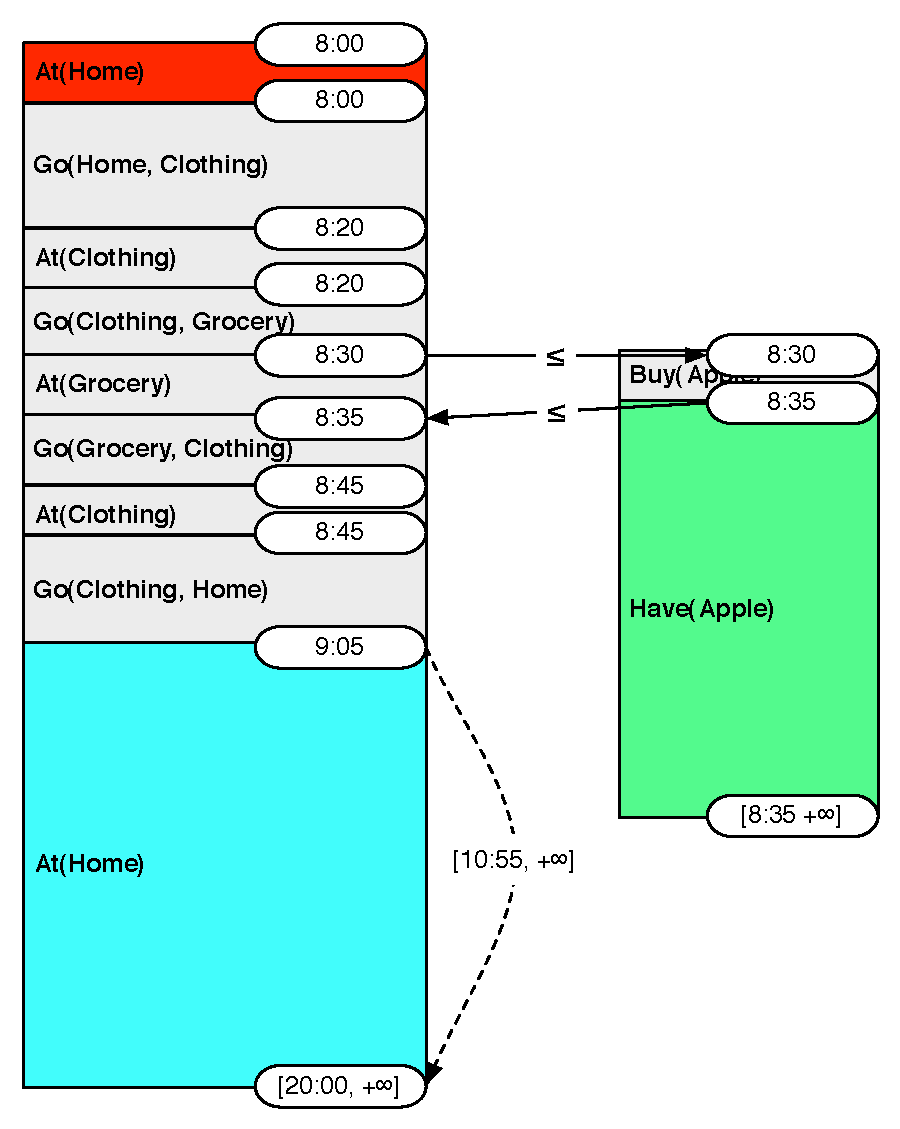
\includegraphics[width=0.65\columnwidth]{figs/example_early}
  \vskip-3mm
  \caption{\small A proactive solution for the plan from
    Fig. \ref{fig:ex:plan} resulting in a Surfacing event at the end
    of mission lasting in excess of $7$ hours.}
  \label{fig:ex:proactive}
  \vskip-5mm
\end{figure}

After analyzing the objectives, we note that these policies are
because of divergent goal semantics. While visiting {\em Vent 1} was
reflecting a \emph{scientific need}, the goal to be back at the
surface is an \emph{operational requirement} to avoid risk due to the
battery running out. While fulfilling both goals are equally important
for mission success, they do not carry the same notion of urgency. It
is desirable for the AUV to visit vents as early as possible but the
motivation to return to the surface is at the end of the mission.
Therefore, a more balanced policy would be to alternate between the
two different approaches depending on what objective(s) the next
action contributes to. The AUV could have been {\em proactive} until
it starts to survey {\em Vent 2} and then {\em defer} heading back to
the surface, continuing to survey the same area, until it either
receives a new goal or the latest start time of the {\em Go} to
\emph{Vent1} action is reached ($\sim$ 17:50). In the event of a new
goal, the resulting mission scenario would then be more efficient in
terms of its \emph{makespan}. We use the latest start time which does
not compensate for uncertainty in the plan and can be easily swapped
with another policy.  Our approach revolves around marking mission
objectives with a policy depending on the exploration of the plan
structure, during plan execution, to identify if the action is linked
to a goal--in which case it needs to be executed 
{\em proactively}--otherwise leading towards a {\em deferred} execution policy for the
action.
 

% We demonstrate a scenario where the AUV ideally uses the two
% approaches at different times. The initial problem is illustrated in Figure
% \ref{fig:Example}.

% The AUV mission starting at 8 AM needs to {\em sample vent2} and
% return to the {\em ship} by 8 PM. The AUV starts traveling immediately
% to {\em vent1}. Considering that that it takes one to two hours to go
% from the {\em Surface} to {\em vent1}, roughly ten minutes to go from
% {\em vent1} to {\em vent2}, and more than two hours in order to {\em
% survey} and {\em sample}, a general plan solution is presented in
% Figure \ref{fig:ex:plan}. The plan presented here is partially
% instantiated giving the AUV the freedom to decide {\em when} to start
% each action within the valid boundary of the solution. For example,
% the AUV should go early in order to {\em sample vent2} so that the
% scientists have the a possibility for requesting more
% tasks. Conversely, heading back to the surface early would waste
% valuable time, roughly two hours, if the scientists decide they want to
% {\em survey} another location. Though by 6pm, it should go to the
% surface so the scientists can pick it up by 8pm. In this scenario, we
% see that the AUV alternated between deciding to execute actions early
% or {\em defer} them depending on the nature of the action it needed to
% take next, or more accurately the nature of the objectives related to
% this action. The AUV was {\em proactive} on traveling to {\em sample vent2}
% because the scientists want it to be completed. On the other hand, the
% AUV has to return to the surface by 8 PM, however, the scientists don't
% explicitly want this done, allowing it to procrastinate.  By
% doing so, the AUV is available to complete new tasks given to it by
% the scientist.\fcomment{One concept that would help if introduced is
%   around the same notion of task span in plan optimization : we have
%   the same problem here but we use a more refined execution policy in
%   order to avoid extraneous actions should a goal come back to us.}



% While this example may appear academic at first, it reflects situations
% we have seen within embedded agent execution in our domain. Indeed, we
% do daily operations wehere our AUV is deployed and scientists can
% remotely send new objectives as the mission goes along to the vehicle
% as they see new areas of interest. Especially in the upper water
% column the nature of the area to be examined depends highly on the
% dynamic of the ocean itself and is difficult to predict beforehand. Therefore,
% scientist can use data sampled by the AUV or other sources (eg
% satellite data, ship based observations, \dots{}) during the beginning of
% the operation in order to give it better informed objectives for the
% rest of the operation. At the same time the vehicle has
% also operational objectives such as going to a place where its
% recovery will be easier for operators. This gives a similar
% distinction between the science objectives and operation
% objectives. Similarly to our example we do not really want the
% AUV to get back to recovery area too early as a new science goal could
% be sent to it which in turn would rather be fulfilled as early as
% possible.

% This paper discusses the problem of dispatching when trying to execute
% a plan. In particular, dispatching in a dynamic environment where the
% plan is expected to change due either to unanticipated events or external
% requests with new directives. External requests  can occur
% at any time which make them in essence uncontrollable events.
% Specifically, we focus on how these new requests, coming from the
% external world, alter the way we need to dispatch the plan, rather than
% how they will be integrated into the plan or any part of the planning
% process. The reason for our separation from planning is that
% oftentimes planning and executing are split up into two different
% jobs. Often times a robotic agent is given an already created plan, and it
% must then choose when to execute parts of the plan. Therefore, our focus is on
% developing a method for dispatch a plan, after it has already been created, while
% understanding that new requests may come in the future.

% The approach we have taken on dispatching looks at the token level of a plan,
% specifically at tokens generated from external requests which we define as goals.
% Because they have been requested by an external person with the intent of being 
% completed promptly, they have a high priority. In contrast, there are tokens that only describe the
% evolution of a timeline, which we define as non-goals. In order to keep the plan 
% valid, the agent is obligated to complete the non-goals, but there is no rush. Thus, the
% non-goals have a low priority. Therefore, we want to complete the goals
% as early as possible in order to give adequate time for the possibility of new
% goals, and complete the non-goals as they become necessary for the validity of the plan. 
% Some may argue that finishing the goals early doesn't guarantee that
% there will be enough time for new goals, however, that is an issue with planning, 
% and our concern is whether dispatching caused the waste of time.


%%% Local Variables: 
%%% mode: latex
%%% TeX-master: "aaai13"
%%% End: 
